\documentclass{beamer}

\usepackage{lipsum}  

\usetheme[progressbar = frametitle]{metropolis}
\setbeamertemplate{frame numbering}[fraction]
\useoutertheme{metropolis}
\useinnertheme{metropolis}
\usefonttheme{metropolis}
\usecolortheme{spruce}
\setbeamercolor{background canvas}{bg = white}

\definecolor{mygreen}{rgb}{.125,.5,.25}


\title{Functions limits derivatives}
%\subtitle{SubTitle here}
\author{}
\institute{\large{\textbf{Conteudo}} \\{6pt \lipsum[1]}}
\date{}


\begin{document}

\metroset{block = fill}

\begin{frame}
\titlepage
\end{frame}

\begin{frame}[t]{Title name of the slide}\vspace{10pt}
    %Hello
    %\begin{block}<>{Definition of a Function}<>
    \begin{block}{Definition of a Function}
        \vspace{0.5em}
        A \textbf{Function} $f$ is a rule that assigns each element $x$ in a set $D$ exactly one element, called $f(x)$ in a set $E$.
        \vspace{0.5em}        
    \end{block}
\vspace{10pt}
Set $D$ is called the 
\only<1>{\line(1,0){50}}
\only<2>{Domain}
\, of the function \\[10pt]

Set $E$ is called the 
\only<1>{\line(1,0){50}}
\only<2>{Range}
\, of the function


\end{frame}


\begin{frame}{Your very first flash card} \vspace{10pt}
    $\sqrt{x^2}=$ \\ [10pt]
    \begin{enumerate}[(A)]
        \item $x$
        \item $-x$
        \item $|x|$
        \item undefined
    \end{enumerate}
\end{frame}

\begin{frame}{Your very first flash card} \vspace{10pt}
    \begin{columns}[onlytextwidth]
        \column{0.5\textwidth}
        $\sqrt{x^2}=$ \\ [10pt]
            \begin{enumerate}[(A)]
            \item $x$
            \item $-x$
            \item $|x|$
            \item undefined
            \end{enumerate}
        \column{0.5\textwidth}
        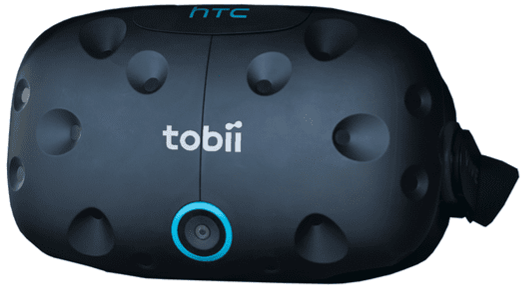
\includegraphics[width = \textwidth]{Introducao/VIVE.png}
    \end{columns}    
\end{frame}



\end{document}